% vim: spell spelllang=en:
%! TEX root = **/00-main.tex

% PCA analysis for numerical variables:

\section{PCA analysis for numerical variables}%
\label{sec:pca_analysis_for_numerical_variables}

% Scree plot. Specify how many principal components are selected
\subsection{Scree plot}%
\label{sub:scree_plot}


\begin{figure}[H]
    \centering
    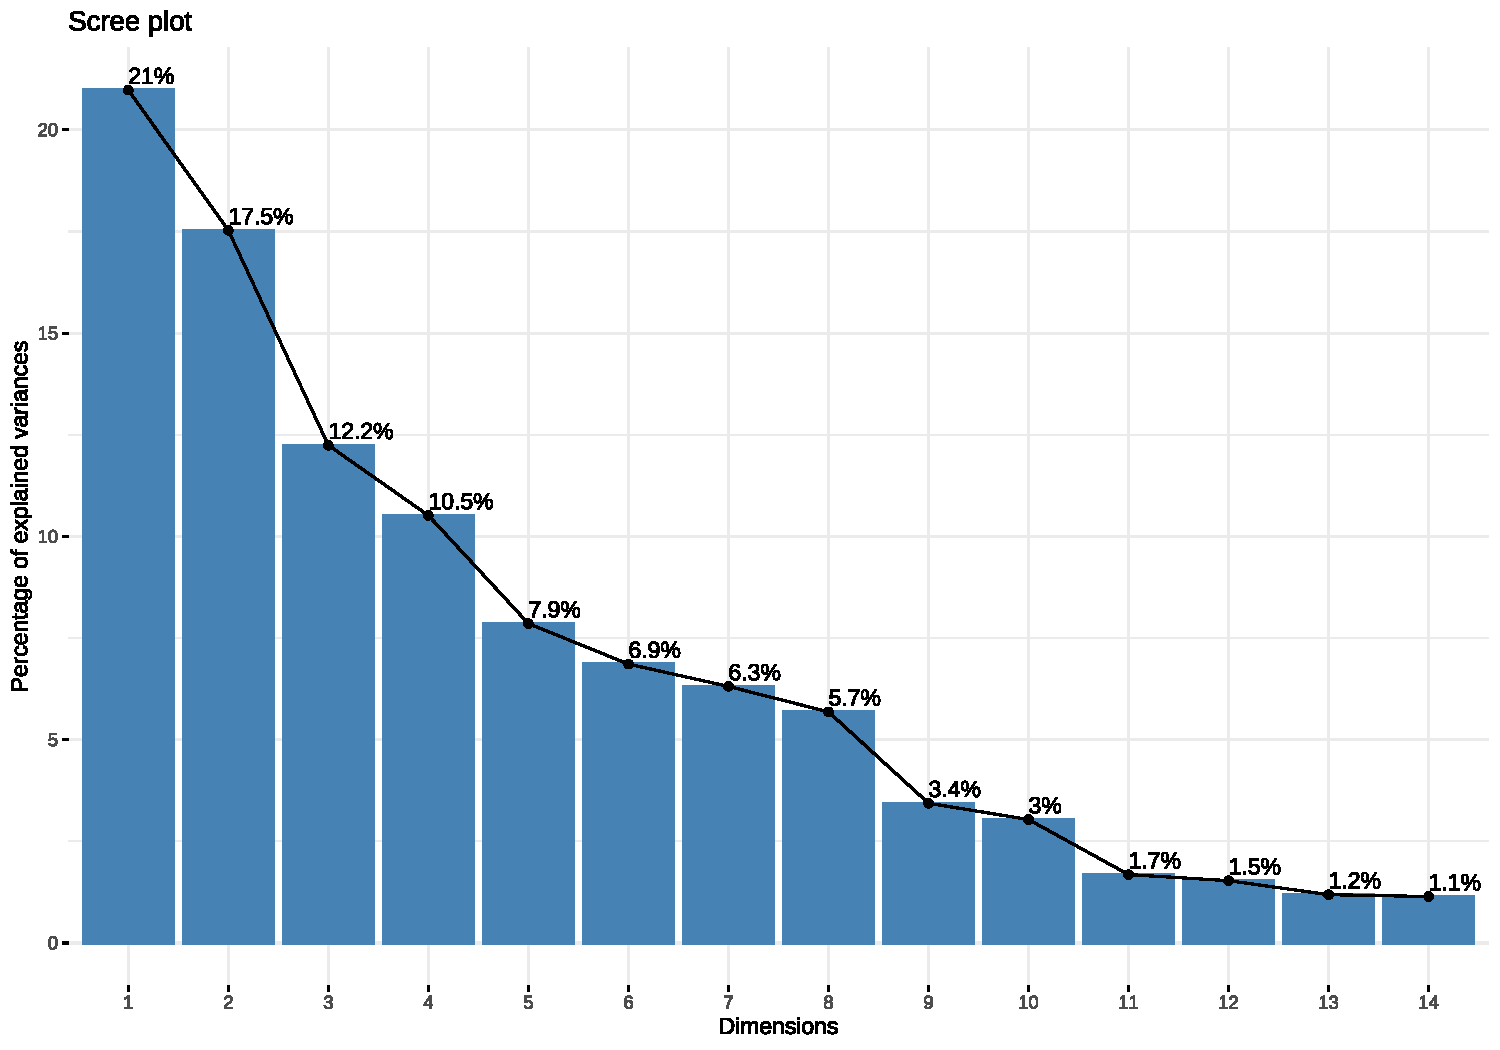
\includegraphics[width=0.7\linewidth]{pca_fact-screeplot} % PCA-inertia_cum
    \caption{PCA inertia}%
    \label{fig:pca_inertia}
\end{figure}

\begin{figure}[H]
    \centering
    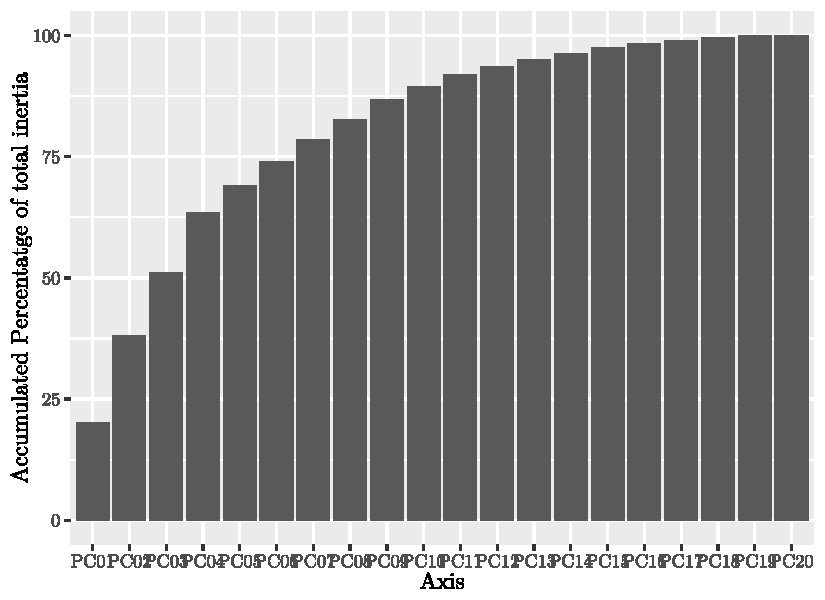
\includegraphics[width=0.7\linewidth]{PCA-inertia_cum}
    \caption{PCA accumulated inertia}%
    \label{fig:pca_inertia_cum}
\end{figure}

\vspace{-1em}
We used the inertia plots to decide the number of factorial axis to analyse. In
\cref{fig:pca_inertia} we can conclude the 4 first axis represent a much
larger amount of variance compared to the others. When looking at
\cref{fig:pca_inertia_cum} we can see that the first 4 axis already contain 63\%
of the variance. If we analyse further with the elbow method we can clearly see
that the slop starts to decrease at around the 4\ts{th} axis. Therefore we decided to
only further analyse the first 4 factorial axis.

% 20.24968405 17.88042469 13.04514781 12.39547495
% 20.24968  38.13011  51.17526  63.57073     %  69.09301  74.04671  78.51992  82.73880


% Factorial map visualisation:
\subsection{Factorial map visualisation}%
\label{sub:factorial_map_visualisation}

% #2 -> caption #3 -> file, #1 -> page
\newcommand{\factorialmap}[2]{
    \begin{figure}[H]
        \centering
        %\includegraphics[trim=3cm 0 3cm 0, clip, width=0.65\linewidth]{plane_#1_#2-var}
        %\parbox[t]{0.24\linewidth}{lorem ipsum dolor sit amet adescipng susisf jsdasj fsdlk ks aksjldsdf jkls}
        \includegraphics[width=\textwidth]{pca_fact-plane_#1_#2-var}
        \caption{PCA plane #1 vs #2}%
        \label{fig:plane_#1-#2}
    \end{figure}
}

\newcommand{\contrib}[2]{
    \begin{figure}[H]
        \centering
        \includegraphics[width=0.85\linewidth]{pca_fact-plane_#1_#2-contrib}
        \caption{PCA variable contributions of plane #1 vs #2}%
        \label{fig:contrib_plane_#1-#2}
    \end{figure}
}

\newcommand{\categorica}[4]{
    \begin{figure}[H]
        \centering
        \includegraphics[width=0.85\linewidth]{pca_fact-#3-plane_#1_#2}
        \caption{PCA variable contributions of #4 in plane #1 vs #2}%
        \label{fig:cat-#3-plane-#1-#2}
    \end{figure}
}

%TODO

\factorialmap{1}{2}

In \cref{fig:plane_1-2} we are showing the factorial maps that represent the most variance among all our factorial axis. When looking at the numerical variables represented we can see that all the variables
related to reviews tend to have similar arrows, this makes sense 
because in the bivariate analysis we concluded that they were correlated.
Looking at \cref{fig:contrib_plane_1-2} we can see that the variables
with higher contribution are the ones about review scores and availability. As all review score variables have a small angle to the first factorial axis we can begin to speculate that this axis is 
mostly affected by these variables. Other variables like availability
and accommodates seem to contribute mostly to the second factorial axis, however these angles aren't as tight so they probably affect the first axis as well.


\factorialmap{1}{3}
In \cref{fig:plane_1-3} we can see that it seems to hold true that 
the review score variables affect axis 1 the most. When looking at accommodates, beds and bedrooms we see that they have similar arrows,
that again makes sense because there is some correlation between them.
These 3 seem to have a much larger contribution to the third factorial axis.

\factorialmap{1}{4}


\factorialmap{2}{3}
\factorialmap{2}{4}
\factorialmap{3}{4}
When looking at \cref{fig:plane_3-4} we can see that the variable arrows seem to group in 3 different groups: the ones regarding number of reviews, the ones about availability and others related to accommodates and bedroom. When looking at \cref{fig:contrib_plane_3-4} we can see
that the ones that contribute the most are bedrooms, accommodates 
and reviews per month. 


\begin{landscape}

\contrib{1}{2}
\contrib{3}{4}

\categorica{1}{2}{room_type}{room type}
\categorica{1}{3}{room_type}{room type}
\categorica{1}{4}{room_type}{room type}

\end{landscape}

% (Be sure you use a single landscape pager for each single map in order to
% guarantee visibility of materials to the readers)

% For each factorial map provide:

% - Individuals projections

% - Common projection of numerical variables and modalities of qualitative
% - variables (take care to use correct color codes as explained along the course)

% - Interpretation of relationships among variables observed. When possible,
% - interpret the latent variable associated with the principal axis

% - Conclusions

% Note: All factorial maps must be placed in a single landscape page that makes
% it visible
